Compared to the initial version of the SG-t-SNE-Pi algorithm in c/c++, the pure julia version of the algorithm 
is lacking. After around 8 threads we encounter diminishing returns. We reached a point where we exceeded 
the physical threads enough to gain minimal to no boost in performance. If we had more physical threads 
we could benefit from assigning more Julia threads to the program. However since we want it to be able to 
run on various hardware and the Julia wrapper highlighted significantly better performance on the same 
hardware, the parallelization of the attraction\_force function would have to change. The following profiling 
proves that attraction\_force is still the most costly process:
\begin{figure}[H]
    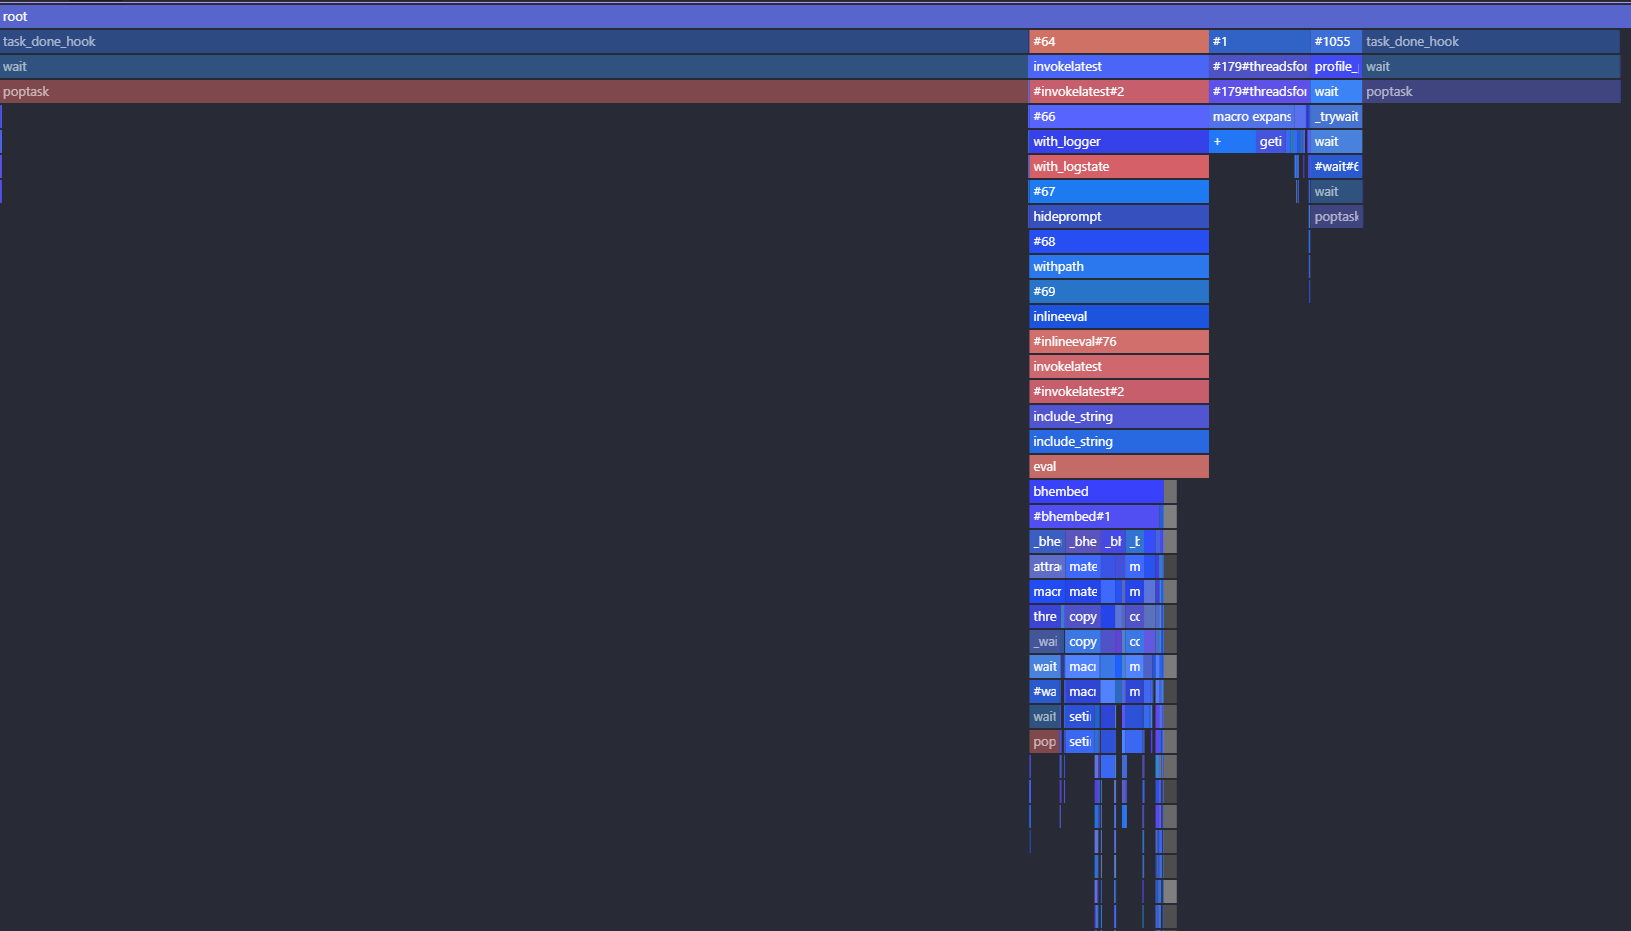
\includegraphics[width=0.5\textwidth]{media/bhembedProfiling.png}
    \caption{Profiling the best pure Julia version}
\end{figure}

To conclude, it seems that the key to advancing the sgtsnepi pure julia project most likely lies in 
finding a better way of parallelizing attraction\_force.